\chapter{Analisi temporale}

\section{Nmap}
In questo capitolo vengono presentati i risultati della comparazione tra le varie istanze di esecuzione fatte con \textit{nmap}, selezionando alternativamente le opzioni precedentemente descritte. L'analisi effettuata è indirizzata sulla durata dell'attacco, il tempo impiegato da Snort per rilevarlo ed il ritardo introdotto dalla rete.

\subsection{Nmap, -A vs Default}
A parte il tempo di rilevamento molto simile, che risulta essere di circa un decimo di secondo più veloce per \textit{nmap -A}, si nota come l'opzione \textit{-A}, rispetto alla versione standard di nmap, faccia uso di molte più operazioni per la scansione delle porte del sistema attaccato, puntando ad effettuare una scansione più esaustiva del normale, come mostrato dai valori di durata dell'attacco.\\
Più intuitivo e chiarificante risulta essere il seguente grafico:\\

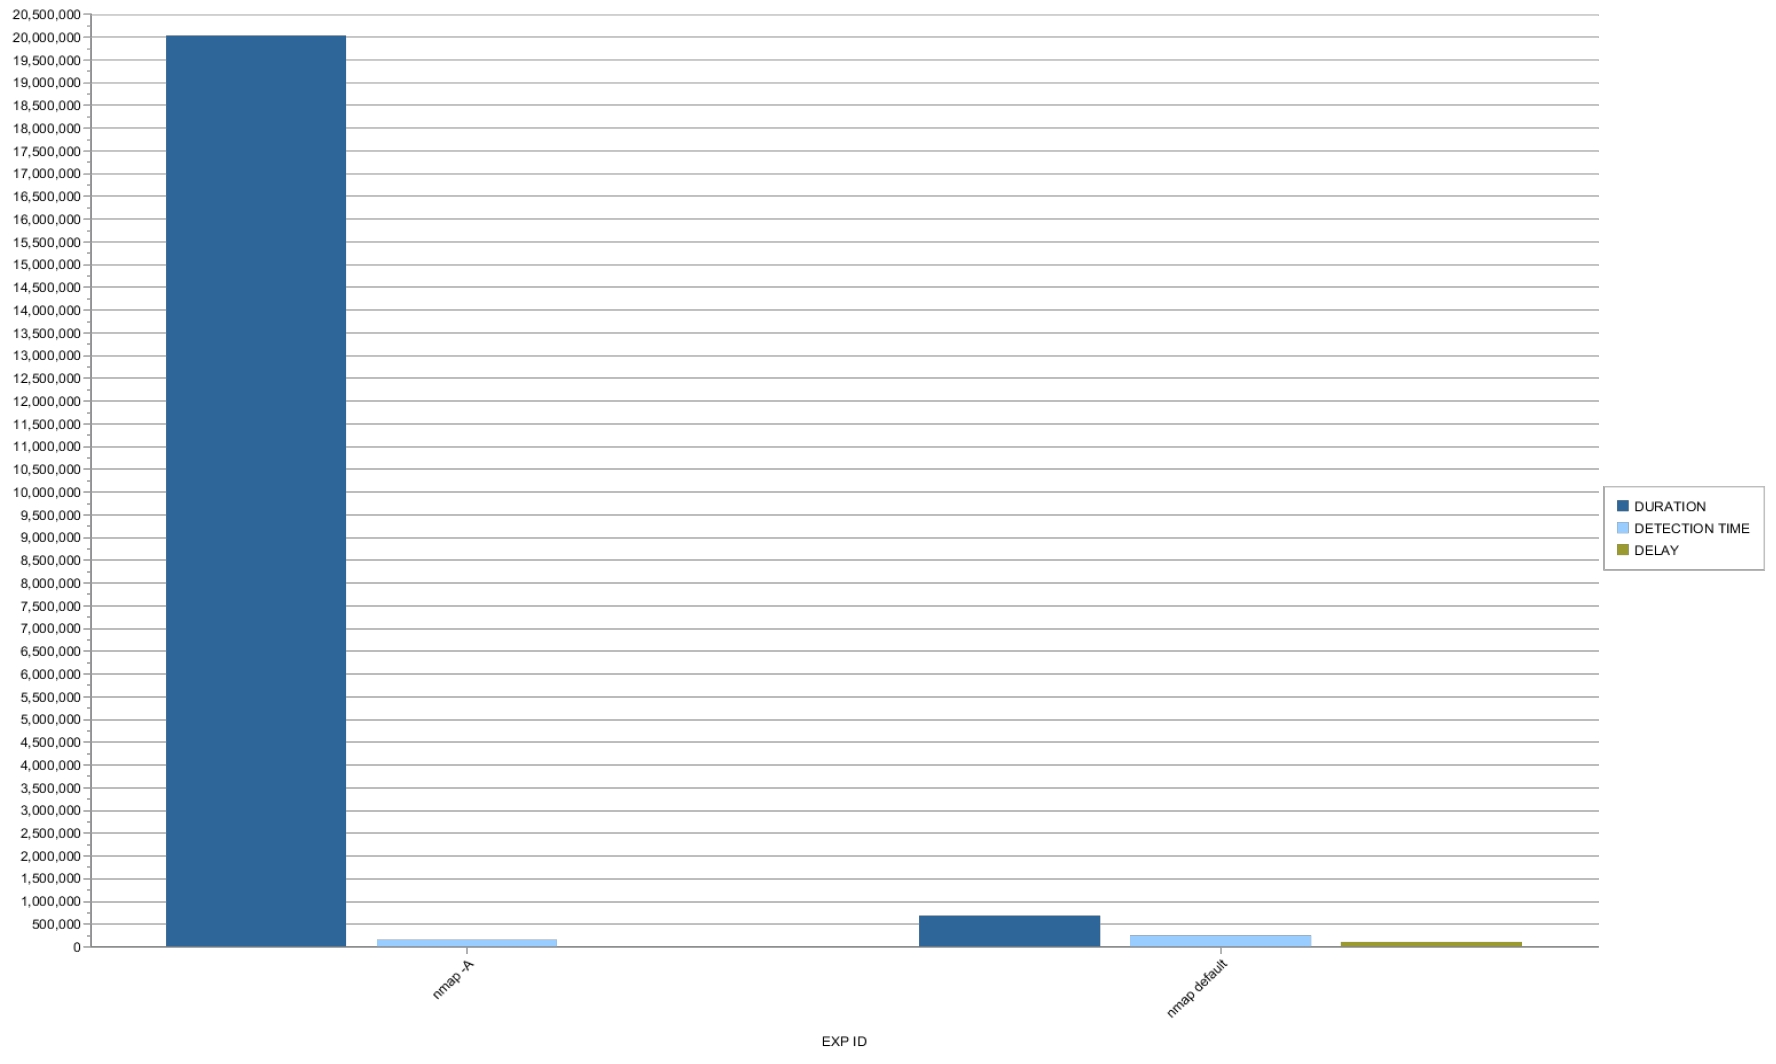
\includegraphics[scale=0.3]{figure/tempi_nmap_A.jpg}\\

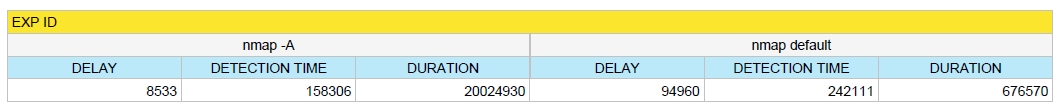
\includegraphics[scale=0.5]{figure/tabella_nmap_A.jpg}

\subsection{Nmap, --osscan-guess vs Default}
Come descritto dal manuale di nmap, utilizzando l'opzione --osscan-guess si esegue un attacco più aggressivo, destinato, quindi, a terminare prima. Snort, come si può vedere dai risultati mostrati dai grafici, riesce a rilevarlo in un tempo più breve rispetto ad una scansione più cauta che quindi passa in principio più inosservata.\\

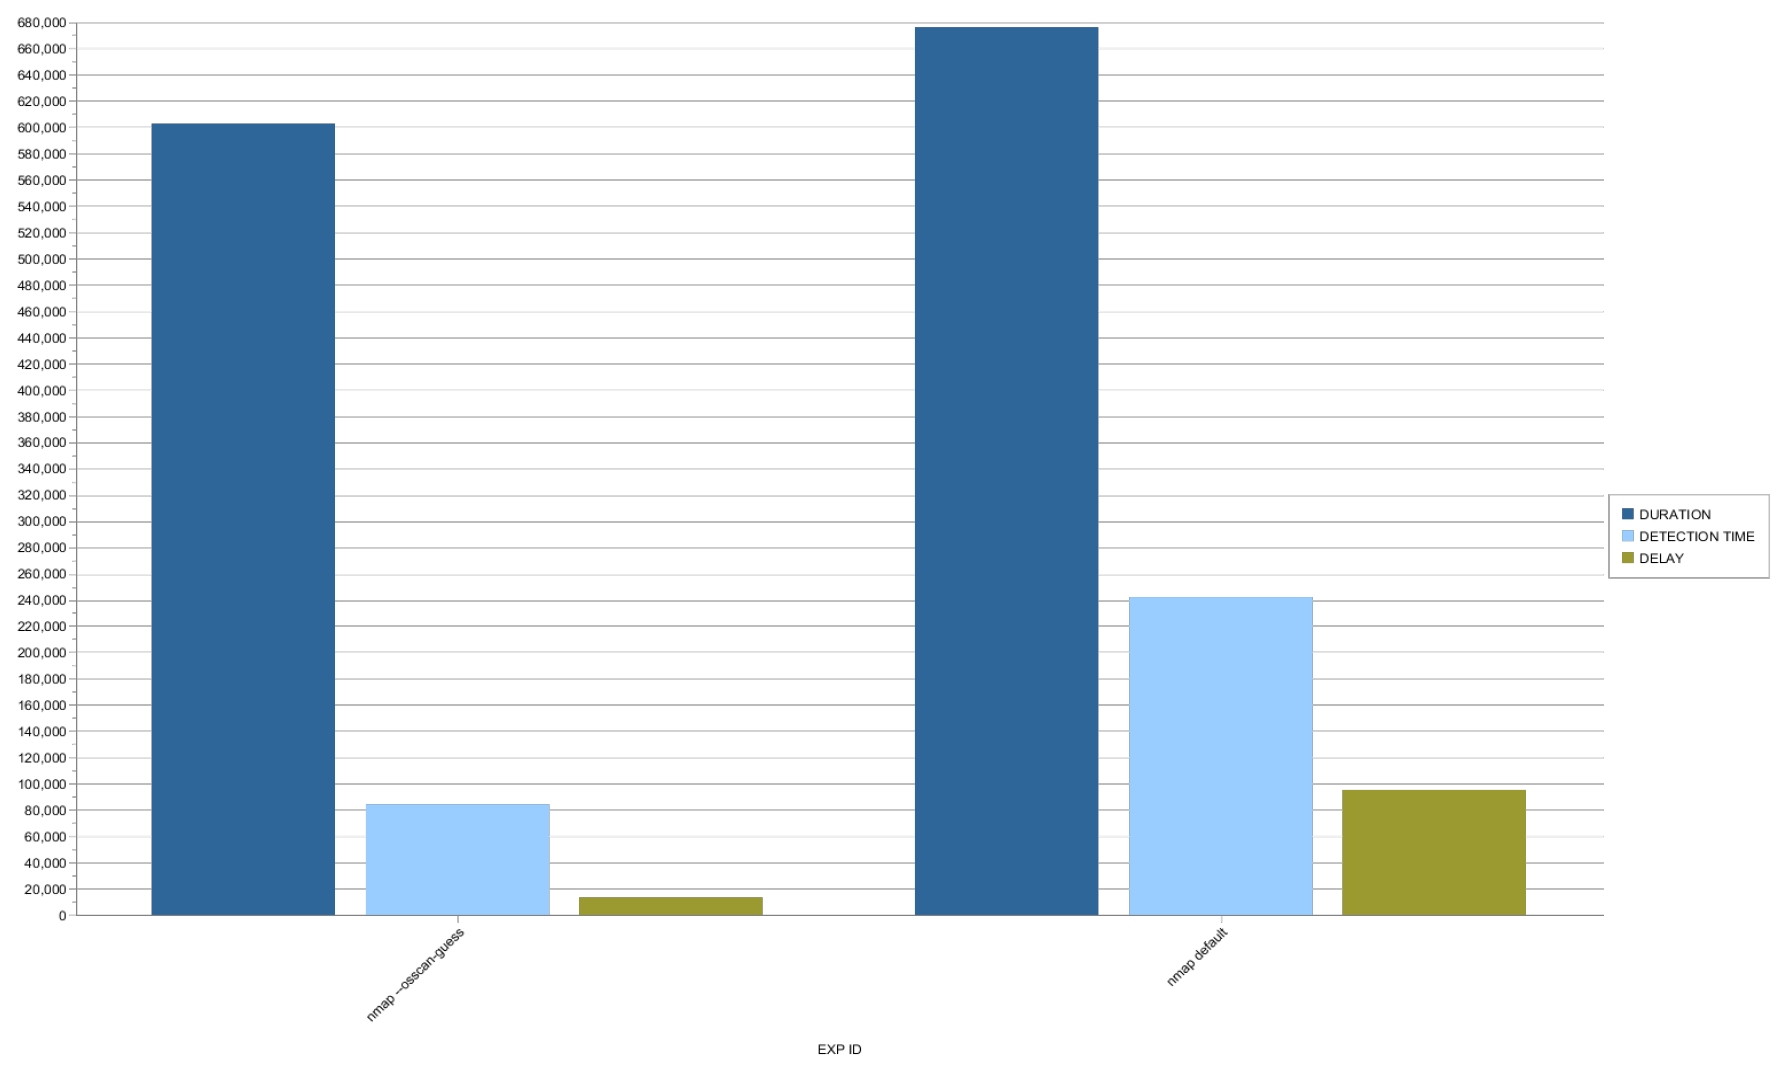
\includegraphics[scale=0.3]{figure/tempi_nmap_osscan.jpg}\\

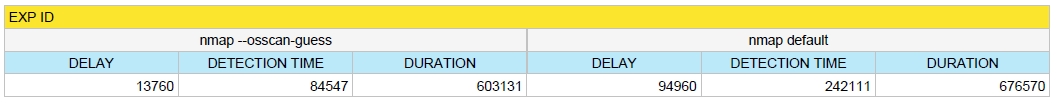
\includegraphics[scale=0.5]{figure/tabella_nmap_osscan.jpg}

\subsection{Nmap, --min-rate 100/300/500 vs Default}
Dalla comparazione dei grafici ottenuti dall'utilizzo di diversi valori (100, 300 e 500 pacchetti/secondo) per l'opzione \textit{--min-rate} del comando nmap possiamo dedurre, intuitivamente, che forzare l'attacco ad inviare più pacchetti al secondo rende l'attacco più veloce e più facilmente rilevabile, dal momento che il numero/tipo di pacchetti necessari a Snort per rilevare l'attacco arrivano con frequenza maggiore. Comparando, inoltre, questi risultati con la versione standard (senza opzioni) di nmap, possiamo ipotizzare che quest'ultima invii i pacchetti necessari ad un rate maggiore di 500 pacchetti/secondo (si vede facilmente seguendo la curva dei tempi di rilevamento). Infine, comparando anche la durata totale dell'attacco, possiamo dedurre che la versione default di nmap esegue più operazioni (o operazioni più complesse) rispetto alla versione che utilizza l'opzione \textit{--min-rate}.\\

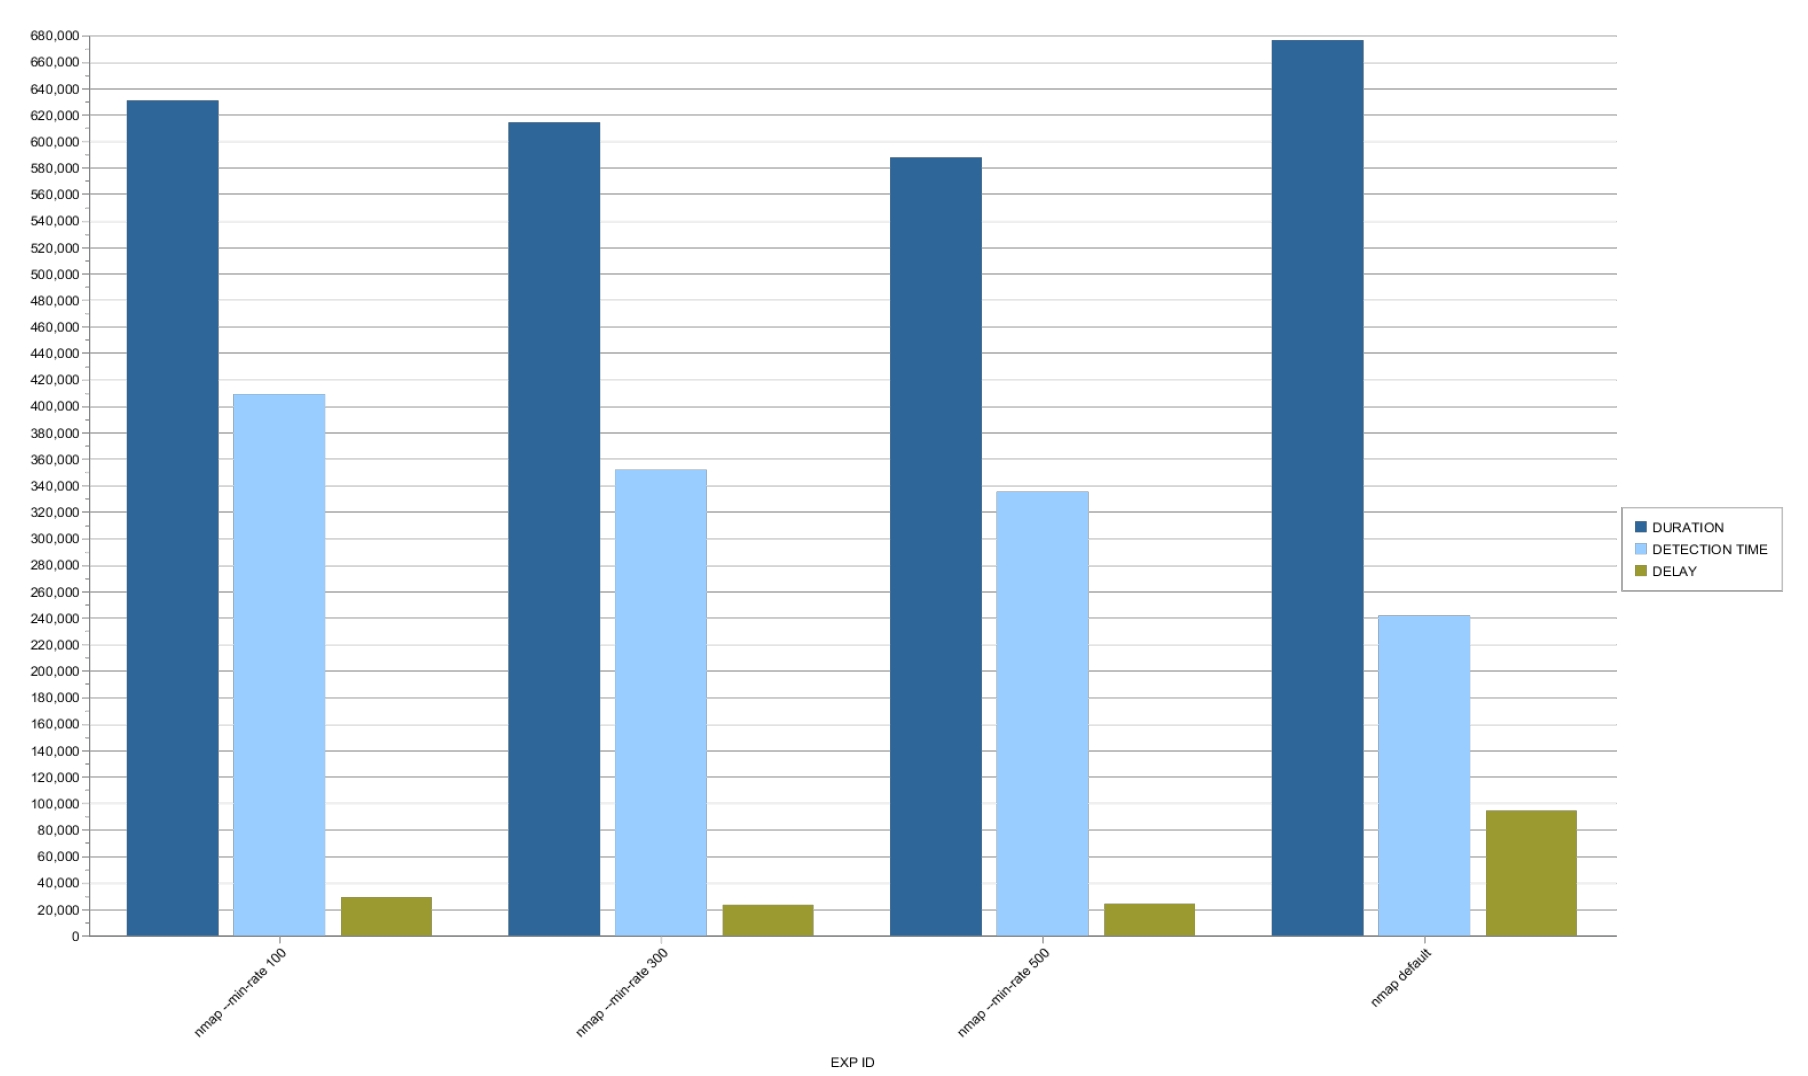
\includegraphics[scale=0.3]{figure/tempi_nmap_minrate.jpg}\\

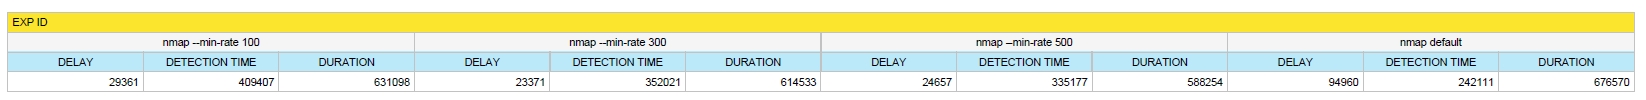
\includegraphics[scale=0.3]{figure/tabella_nmap_minrate.jpg}

\subsection{Nmap, -T 2/3/4/5 vs Default}
Notiamo innanzitutto come le tempistiche di durata e di rilevamento per l'attacco "educato" di nmap (per comodità visualizzato in un grafico a parte) siano fuori scala rispetto a tutti gli altri timing templates. Questo tipo di attacco è infatti stato progettato per agire lentamente, cercando di ridurre al minimo ogni possibile rilevamento da parte di un ipotetico IDS. Per quanto riguarda gli altri templates, possiamo dedurre che l'attacco "aggressivo" (\textit{-T4}) è probabilmente il miglior punto d'incontro tra velocità d'attacco e furtività, permettendo una rapida scansione in grado di aggirare per breve tempo un generico IDS.\\

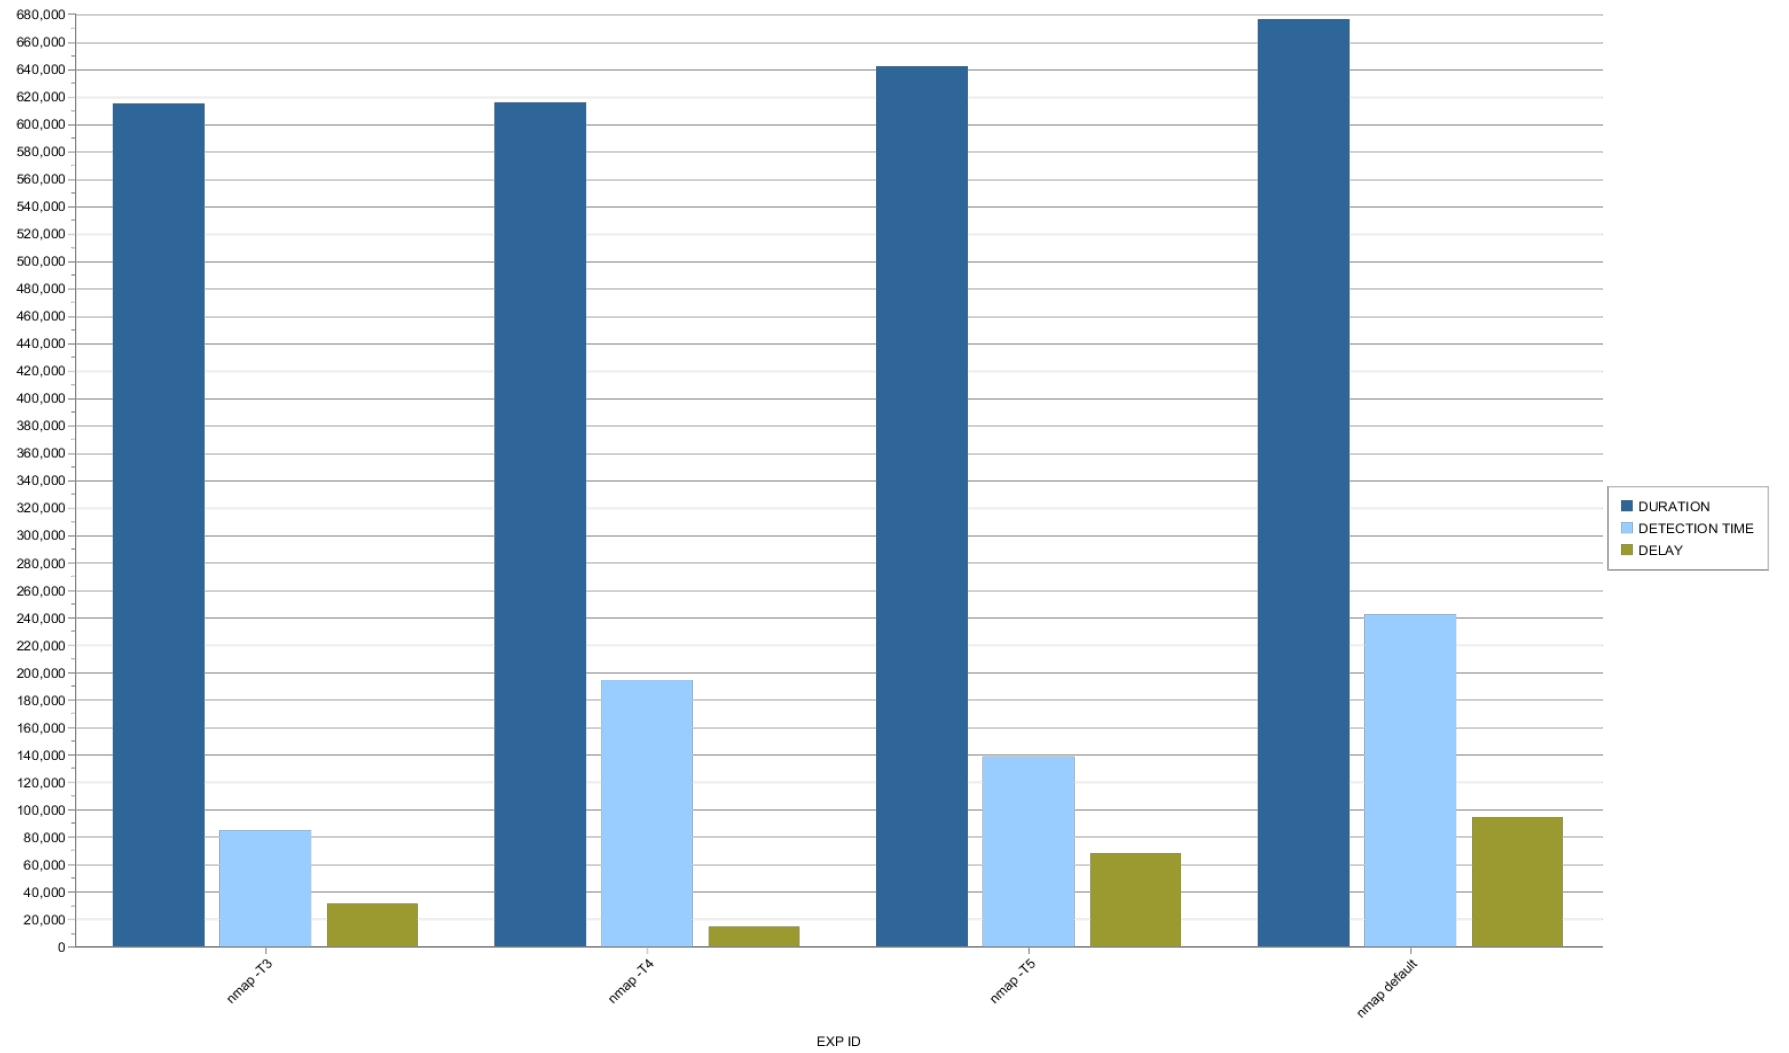
\includegraphics[scale=0.3]{figure/tempi_nmap_T.jpg}\\

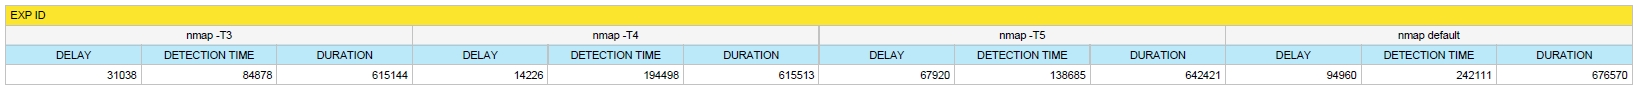
\includegraphics[scale=0.3]{figure/tabella_nmap_T.jpg}\\

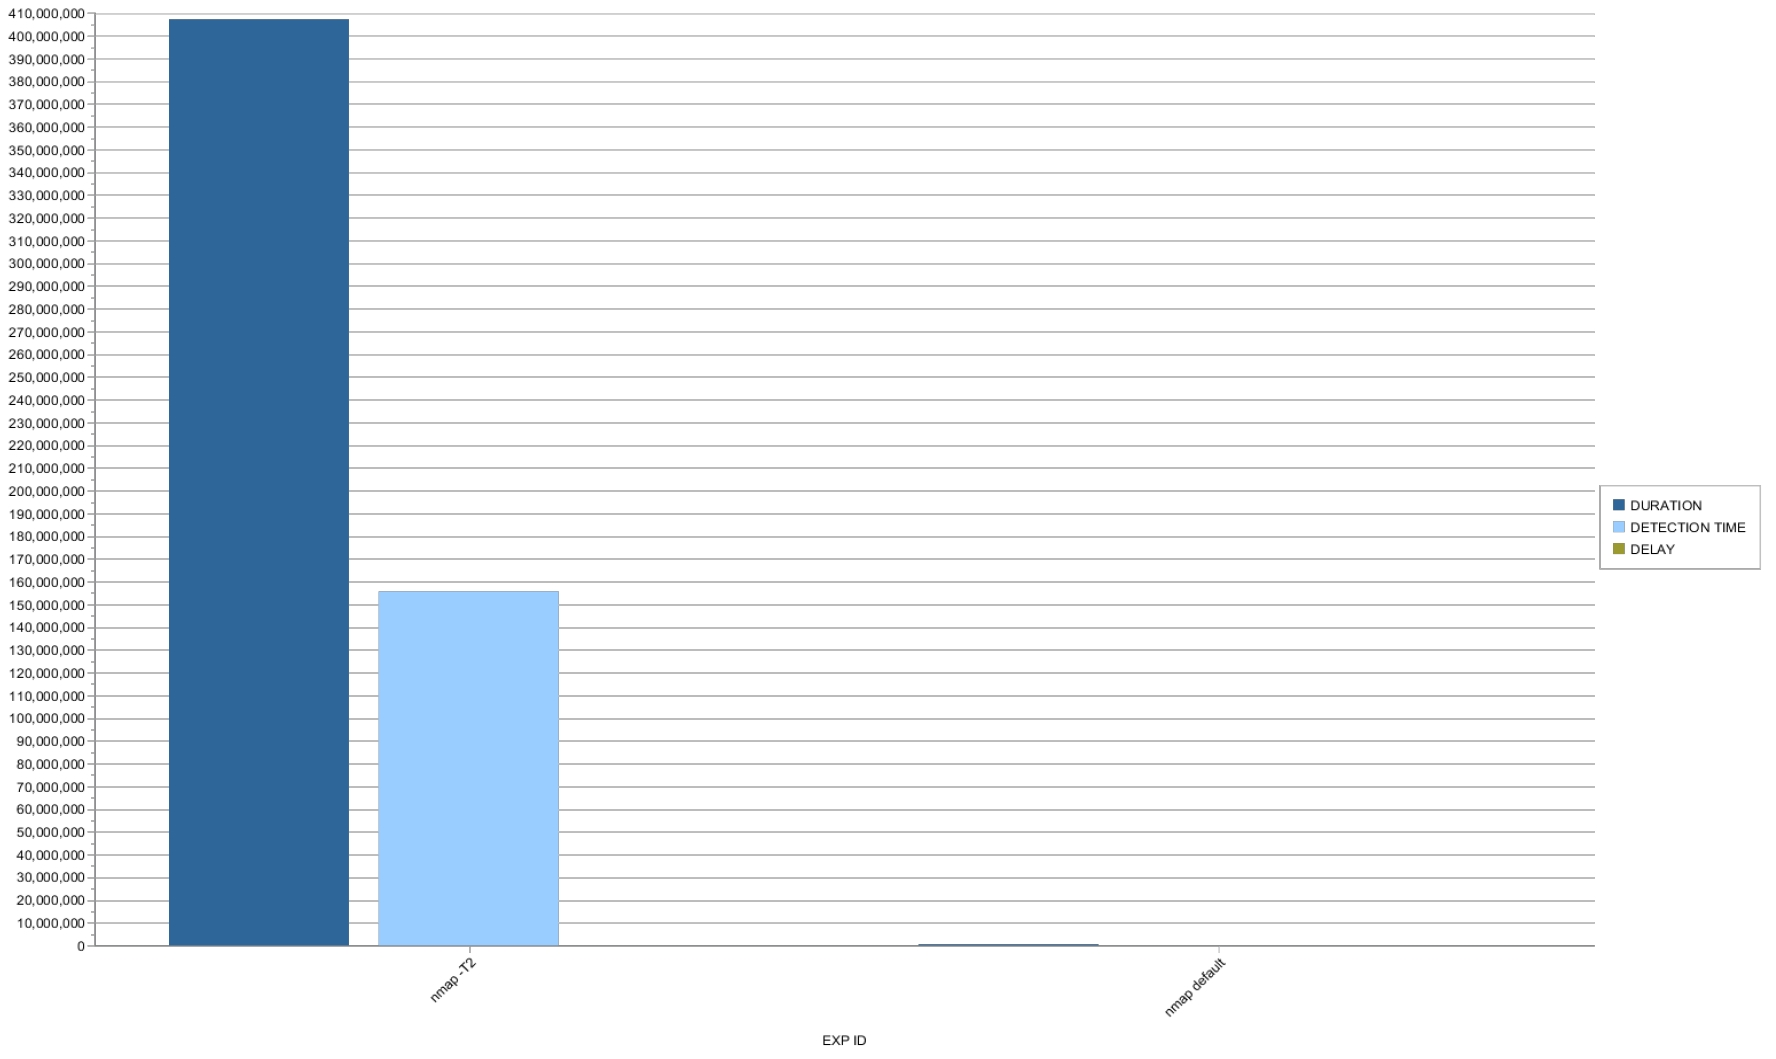
\includegraphics[scale=0.3]{figure/tempi_nmap_T2.jpg}\\
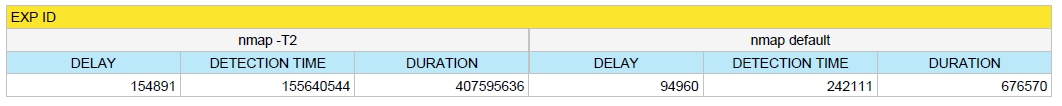
\includegraphics[scale=0.4]{figure/tabella_nmap_T2.jpg}

\subsection{Nmap, --version-all/light vs Default}
Osservando il grafico seguente, ed in particolare le colonne relative al tempo di detection dell'attacco, si vede subito come la versione leggera (\textit{--version-light}) sia più velocemente riconoscibile da un IDS come Snort rispetto alla sua controparte esaustiva (\textit{--version-all}). Confrontando questi risultati con la versione standard di nmap possiamo inoltre supporre che quest'ultima sia formata da un tradeoff delle versioni light e all, in quando il suo tempo di rilevazione si trova più o meno tra i due sopra citati.\\

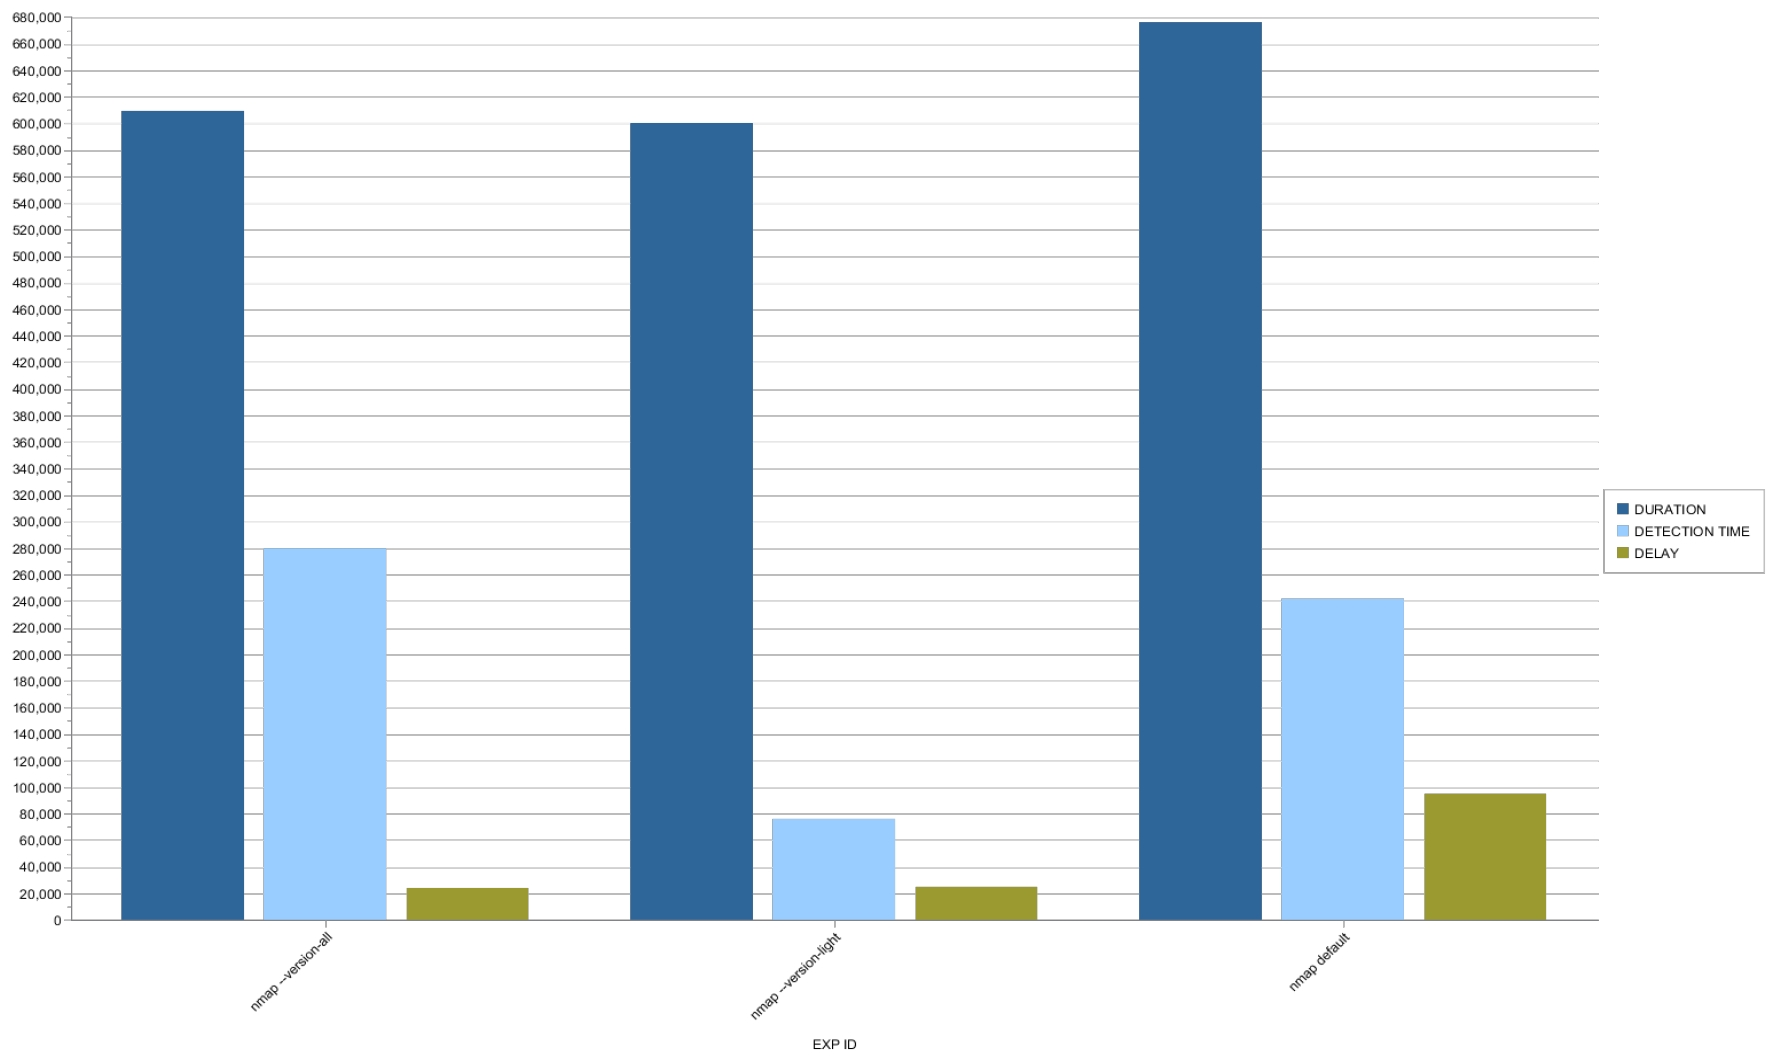
\includegraphics[scale=0.3]{figure/tempi_nmap_all-light.jpg}\\

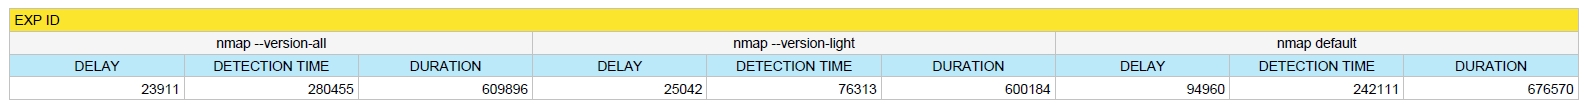
\includegraphics[scale=0.3]{figure/tabella_nmap_all-light.jpg}
